\documentclass[a4paper]{article}

%% Language and font encodings
\usepackage[french]{babel}
\usepackage[utf8x]{inputenc}
\usepackage[T1]{fontenc}

%% Sets page size and margins
\usepackage[a4paper,top=3cm,bottom=3cm,left=2cm,right=2cm,marginparwidth=2cm]{geometry}
%% Useful packages
\usepackage{amsmath}
\usepackage{graphicx}
\usepackage[colorinlistoftodos]{todonotes}
\usepackage[colorlinks=true, allcolors=black]{hyperref}
\usepackage{fourier-orns}
\usepackage{titlesec}
\usepackage{fancyhdr}
\usepackage{fancyvrb}
%\renewcommand{\thefootnote}{\*}
\pagestyle{fancy} 
\setcounter{tocdepth}{5}
\usepackage{float}
\usepackage{subcaption}


%% Tikz stuff
\usepackage{tikz}
\usetikzlibrary{calc, arrows}
\tikzstyle{incolore} = [rectangle, rounded corners, draw=black, minimum height=1cm, minimum width=3cm, text width=3cm, text centered]


\usepackage{libertine}
\newcommand{\hsp}{\hspace{20pt}}
\newcommand{\HRule}{\rule{\linewidth}{0.5mm}}


\renewcommand{\headrulewidth}{1pt}
\fancyhead[C]{} 
\fancyhead[L]{}
\fancyhead[R]{\footnotesize{\leftmark}}

\renewcommand{\footrulewidth}{1pt}
\fancyfoot[C]{} 
\fancyhead[L]{}
\fancyfoot[R]{\thepage}

\definecolor{Zgris}{rgb}{0.87,0.85,0.85}

\usepackage{eso-pic,graphicx}
\usepackage{xcolor}
\newcommand{\bgimg}[1]{
\AddToShipoutPicture
   {
      \put(\LenToUnit{0 cm},\LenToUnit{0 cm})
      {
            \includegraphics[width=\paperwidth,height=\paperheight]{#1} 
      }
   }
}
\begin{document}




%%\bgimg{Image_15.jpg}

















\begin{titlepage}
  \begin{sffamily}
  \begin{center}
    % Upper part of the page. The '~' is needed because \\
    % only works if a paragraph has started.
    
\includegraphics[width=5cm]{LogoHenallux.PNG}~\\[1.5cm]
    \textsc{\Large Rapport de laboratoire}\\[1.5cm]
    % Title
    \HRule \\[0.4cm]
    { \huge \bfseries Deuxième laboratoire: Effet Doppler et câblage\\[0.4cm] }
    \HRule \\[2cm]
    % Author and supervisor
    \begin{minipage}{0.4\textwidth}
      \begin{flushleft} \large
        Roumache Grégoire\\
        Sénéchal Julien\\
        Robert Alexandre\\
        Wallemme Maxime\\
        Kenmeugne Lionel\\
        Didion Charles
      \end{flushleft}
    \end{minipage}
    \begin{minipage}{0.55\textwidth}
      \begin{flushright} \large
    	Laboratoire de sciences appliquées à l'informatique\\
		Sécurité des systèmes, technologie de l'informatique\\
		Première année, groupe H \\
		Hénallux\\
		Année académique 2019-2020\\
      \end{flushright}
    \end{minipage}
    \vfill
    % Bottom of the page
    {\large 5 Mars 2020}
  \end{center}
  \end{sffamily}
\end{titlepage}







\let\cleardoublepage\clearpage















\section{Introduction}





Dans le cadre du second laboratoire de Sciences appliquée en première technologie de l’informatique et sécurité des systèmes, nous avons réalisé deux manipulations.

Pour la première, il s’agit d’une manipulation sur l’effet Doppler. Notre but était de mesurer les fréquences émises à différentes vitesses. Nous pouvions ainsi calculer la vitesse du chariot et également la mesurer pour les comparer. Ensuite, pour la deuxième manipulation dont le sujet était le câblage. Nous avons utilisé un testeur de câble et des câbles Ethernet. Nous avons testé si ils fonctionnaient ou non.

Enfin, lors de ce rapport, nous commencerons par éclaircir certains points à l’aide d’un bref rappel théorique afin de comprendre explicitement les manipulations illustrées et expliquées en détails par la suite. 















\section{Rappels théoriques}










\subsection{Effet Doppler}





Lorsque la distance entre l'émetteur et le récepteur d'une onde sonore est constante, alors si la source émet une onde de 40 kHz, le récepteur reçoit une onde de 40 kHz. Mais quand l'émetteur et le récepteur ne vont pas à la même vitesse, l'onde sonore n'aura pas la même fréquence pour l'émetteur et pour le récepteur. Ce phénomène est appelé l'effet Doppler.

Cet effet est illustré dans la figure \ref{fig:dopplerMouvement} où l'on peut voir que les récepteurs au repos qui se trouvent de part et d'autre de la source en mouvement ne mesurent pas la même fréquence d'onde. En comparaison dans la figure \ref{fig:dopplerRepos}, quand la source et les récepteurs sont tous au repos, les émetteurs mesurent la même fréquence.

\begin{center}
    \begin{figure}[H]
        \centering
        \begin{tikzpicture}

            \node [] at (0,0) {Source};
            \node [incolore] at (-6,0) {Récepteur 1};
            \node [incolore] at (6,0) {Récepteur 2};

            \draw (0,0) circle (0.75 cm);
            \draw (0,0) circle (1.25 cm);
            \draw (0,0) circle (1.75 cm);

            \draw (0,0) circle (2.25 cm);
            \draw (0,0) circle (2.75 cm);

            \draw [->] (-7.5,-3.2) -- (-7.5,-0.8);
            \draw [->] (-7.5,-2) -- (3.30-7.5,-2);
            \draw [thick, domain=0:pi, red] plot (\x-7.5,{sin(\x r * 3) - 2});

            \draw [->] (4.5,-3.2) -- (4.5,-0.8);
            \draw [->] (4.5,-2) -- (3.30+4.5,-2);
            \draw [thick, domain=0:pi, red] plot (\x+4.5,{sin(\x r * 3) - 2});

        \end{tikzpicture}
        \caption{Une source et deux récepteurs au repos.}
        \label{fig:dopplerRepos}
    \end{figure}

    \begin{figure}[H]
        \centering
        \begin{tikzpicture}
    
            \node [] at (1,0) {Source};
            \node [incolore] at (-6,0) {Récepteur 1};
            \node [incolore] at (6,0) {Récepteur 2};
    
    
            \draw (1,0) circle (0.75 cm);
            \draw (1-0.25,0) circle (1.25 cm);
            \draw (1-0.5,0) circle (1.75 cm);
    
            \draw (1-0.75,0) circle (2.25 cm);
            \draw (1-1,0) circle (2.75 cm);
    
    
    
            \draw [->] (-7.5,-3.2) -- (-7.5,-0.8);
            \draw [->] (-7.5,-2) -- (3.30-7.5,-2);
            \draw [thick, domain=0:pi, red] plot (\x-7.5,{sin(\x r * 2) - 2});
    
            \draw [->] (4.5,-3.2) -- (4.5,-0.8);
            \draw [->] (4.5,-2) -- (3.30+4.5,-2);
            \draw [thick, domain=0:pi, red] plot (\x+4.5,{sin(\x r * 4) - 2});
    
        \end{tikzpicture}
        \caption{Une source en mouvement et deux récepteurs au repos.}
        \label{fig:dopplerMouvement}
    \end{figure}
\end{center}










\subsection{Câble} \label{subsec:cables}





Les câbles Ethernet que nous avons utilisés dans ce laboratoire étaient soit des câbles droits soit des câbles croisés. La différence entre ces deux types de câbles est mieux expliquée à l'aide d'images. Ainsi, la figure \ref{fig:cableDroit} représente un câble droit alors que la figure \ref{fig:cableCroise} représente un câble croisé.
\footnote{Source des figures \ref{fig:cableDroit} et \ref{fig:cableCroise}: \texttt{https://networkcorp.fr/cable-rj45/}.}

\begin{center}
    \begin{figure}[H]
        \centering
        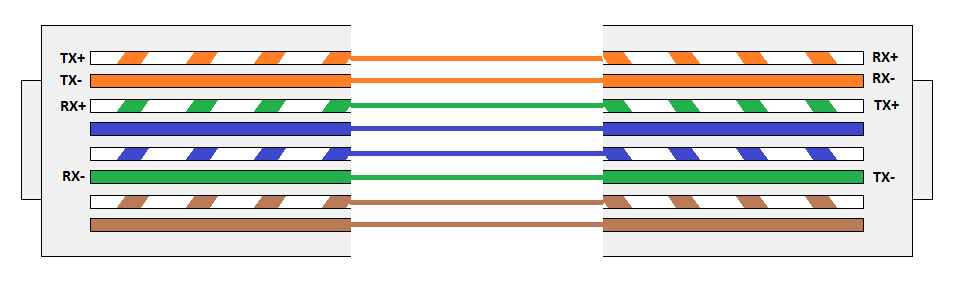
\includegraphics[width=0.85\textwidth]{cable-droit.png}
        \caption{Schéma d'un câble droit.}
        \label{fig:cableDroit}
    \end{figure}
    
    \begin{figure}[H]
        \centering
        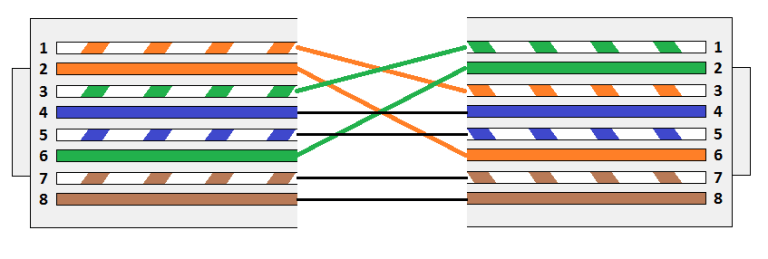
\includegraphics[width=0.85\textwidth]{cable-croise.png}
        \caption{Schéma d'un câble croisé.}
        \label{fig:cableCroise}
    \end{figure}
\end{center}















\section{Manipulation pratique}










\subsection{Effet Doppler}









\subsubsection{Principe de la manipulation}





Il a été question pour nous au bout de cette manipulation d’observer et étudier les décalages de fréquence des ondes entres les mesures à l’émission et à la réception, lorsque la distance entre l’émetteur et le récepteur varie au cours du temps.

Tout d’abord nous avons procéder au montage de notre pack Effet Doppler, par la suite nous avons déterminé la fréquence d’émission et la vitesse du chariot.










\subsubsection{Matériel utilisé}





\begin{itemize}
  \item L’émetteur et récepteur Moduson : ce sont des appareils qui ont pour but de mettre en évidence la nature vibratoire d’un ultrason, mesurer sa période et sa fréquence.
  \begin{figure}[H]
    \centering
    \begin{minipage}{.5\textwidth}
      \centering
      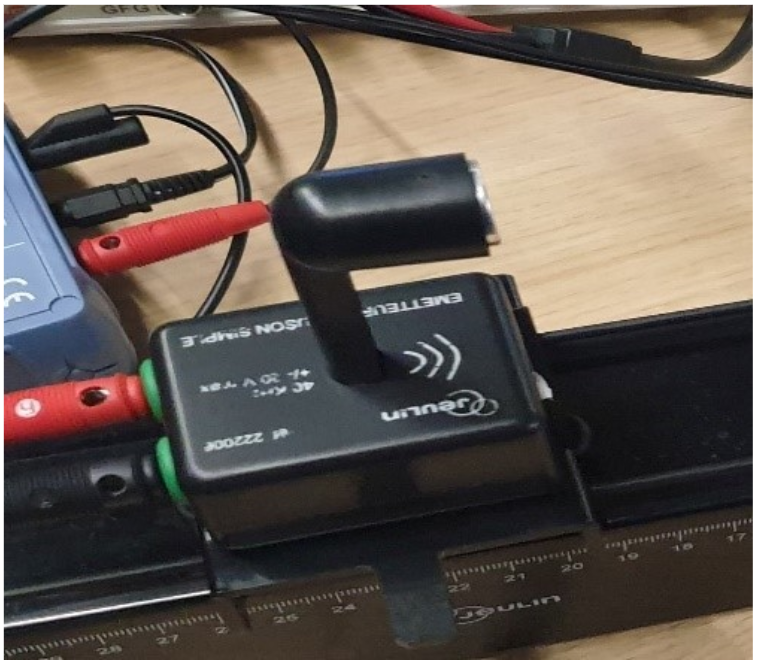
\includegraphics[height=7cm]{emetteur-moduson1.PNG}
      \caption{Émetteur Moduson.}
      \label{fig:emetteurModuson}
    \end{minipage}%
    \begin{minipage}{.5\textwidth}
      \centering
      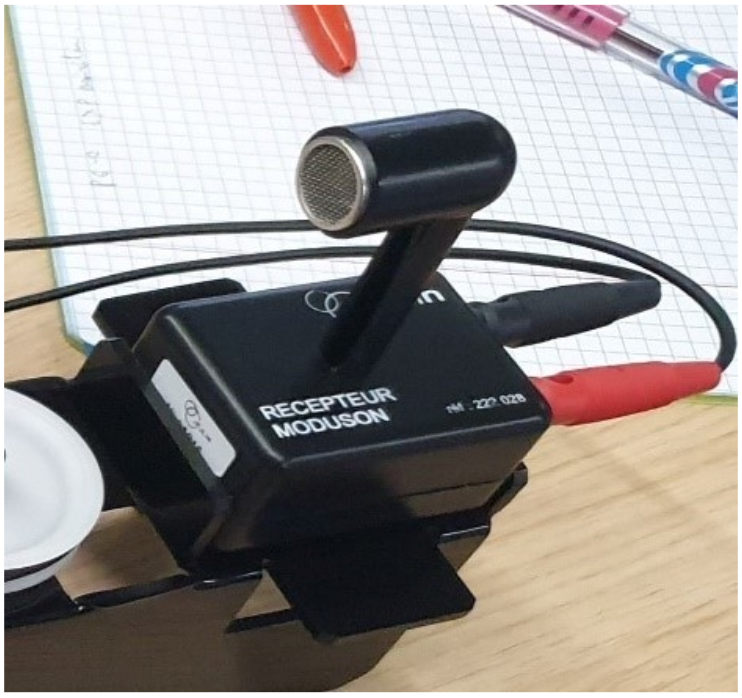
\includegraphics[height=7cm]{recepteur-moduson1.PNG}
      \caption{Récepteur Moduson.}
      \label{fig:recepteurModuson}
    \end{minipage}
  \end{figure}
  \item Câble banane : nous en avons utilisé 8 au total pour connecter les différents outils de notre manipulation entre eux.
  \begin{figure}[H]
    \begin{subfigure}{.5\textwidth}
      \centering
      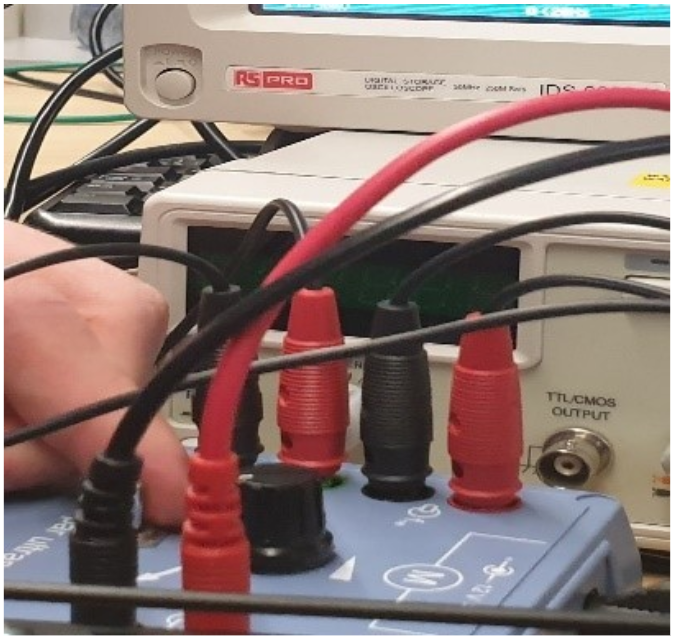
\includegraphics[height=5cm]{cable-banane1.PNG}
      \caption{}
    \end{subfigure}%
    \begin{subfigure}{.5\textwidth}
      \centering
      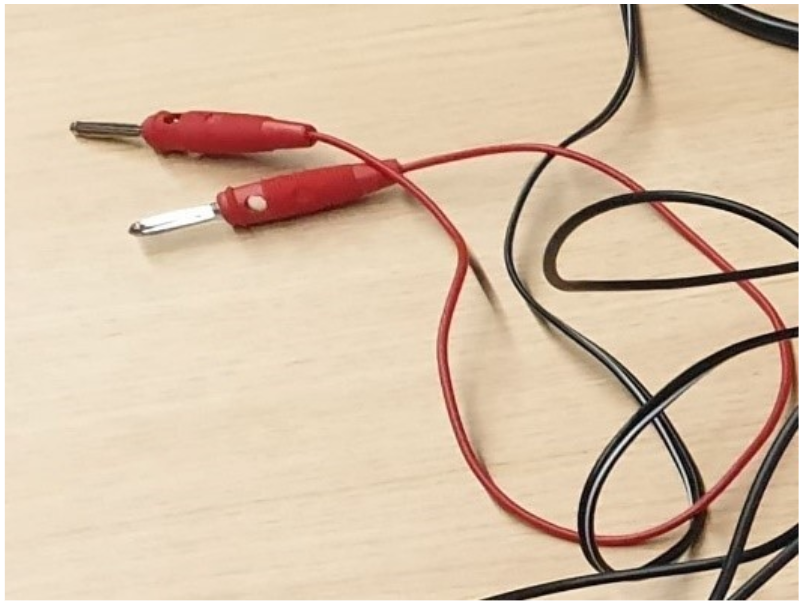
\includegraphics[height=6cm]{cable-banane2.PNG}
      \caption{}
    \end{subfigure}
    \caption{Câbles bananes.}
    \label{fig:cablesBanane}
    \end{figure}
  \item Oscilloscope : c’est l’appareil de mesure qui nous a permis de visualiser les différentes variations de signaux.
  \begin{figure}[H]
    \centering
    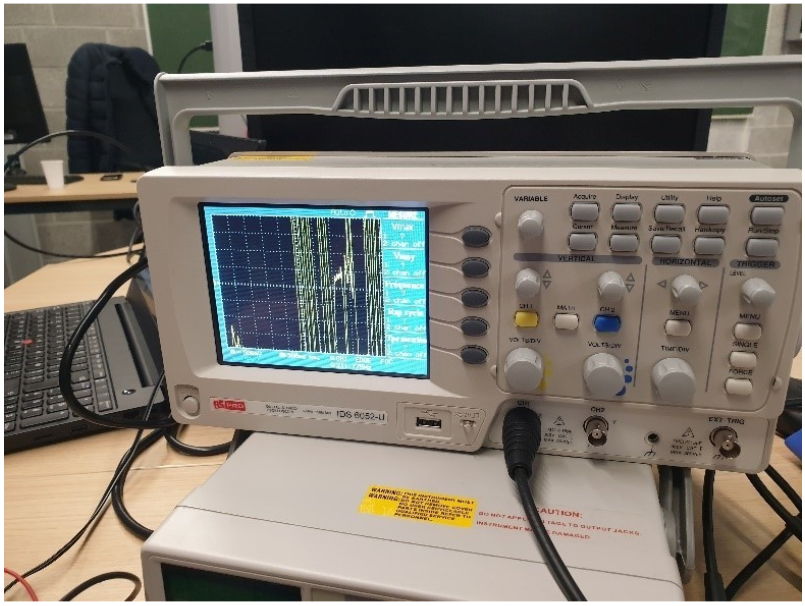
\includegraphics[width=0.85\textwidth]{oscilloscope.PNG}
    \caption{Oscilloscope.}
    \label{fig:oscilloscope}
  \end{figure}
  \item Fourche chronociné : malgré qu’il soit absent lors de notre manipulation car il ne nous a pas été fournie, la fourche chronociné permet de détecter le passage d'un mobile ou d'une bille tout en mesurant sa vitesse, permet de mesurer la vitesse quasi instantanée des objets et le temps de passage à quelques micro-secondes près.
  \begin{figure}[H]
    \centering
    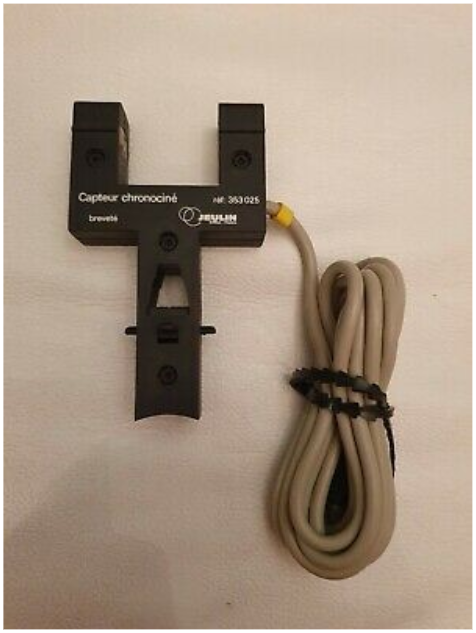
\includegraphics[width=0.4\textwidth, angle=90]{fourche-chronocine1.PNG}
    \caption{Fourche chronociné.}
    \label{fig:fourcheChronocine}
  \end{figure}
  \item Banc mécanique Doppler (figure \ref{fig:quarantecm}) : ce banc motorisé nous a permis de générer le déplacement d'un chariot à vitesse constante et réglable.
  \item Boitier Doppler par ultra son : ce boîtier nous a permis d'obtenir le décalage entre les signaux émis et reçus.
  \begin{figure}[H]
    \centering
    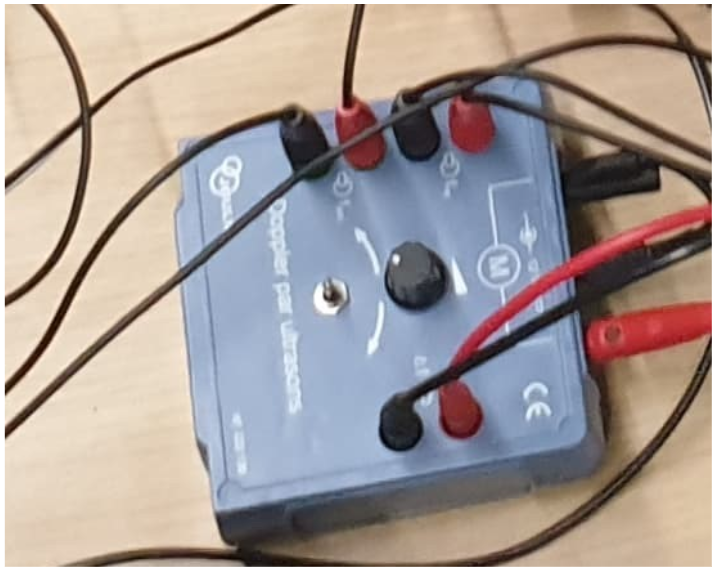
\includegraphics[width=0.7\textwidth]{boitier-doppler.PNG}
    \caption{Boitier Doppler par ultra son.}
    \label{fig:boitierDoppler}
  \end{figure}
\end{itemize}










\subsubsection{Montage et déroulement de la manipulation}





\begin{enumerate}
  \item Nous avons commencé par alimenter l’émetteur Moduson en le branchant sur les bornes vertes à l’aide des câbles banane sur le boitier Doppler par ultrasons, lui-même alimenté à l’aide du bloc alimentation qui nous a été fourni.
  \begin{figure}[H]
    \centering
    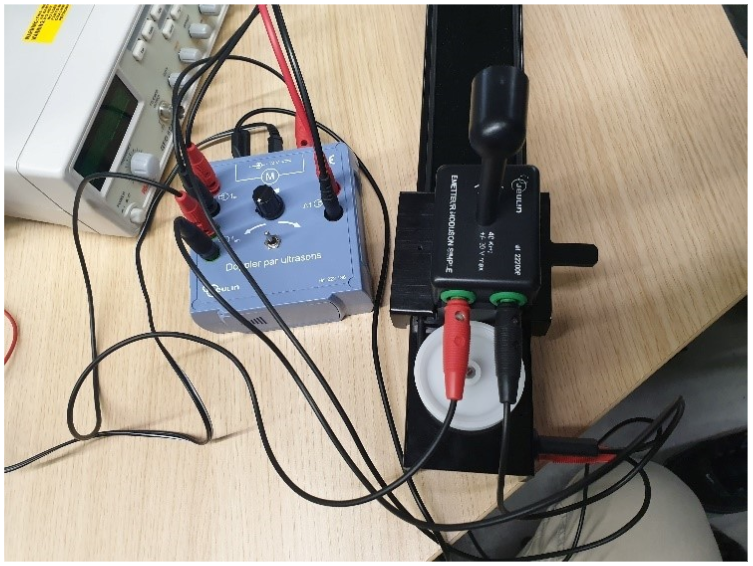
\includegraphics[width=0.7\textwidth]{montage-complet1.PNG}
    \caption{Câblage du montage.}
    \label{fig:cablageDoppler}
  \end{figure}
  \item Puis nous avons branché le récepteur Moduson sur notre oscilloscope, toujours à l’aide de nos câble banane.
  \item Ensuite après avoir placé notre émetteur et notre récepteur en face sur le boitier, on a obtenu le résultat.
  \begin{figure}[H]
    \centering
    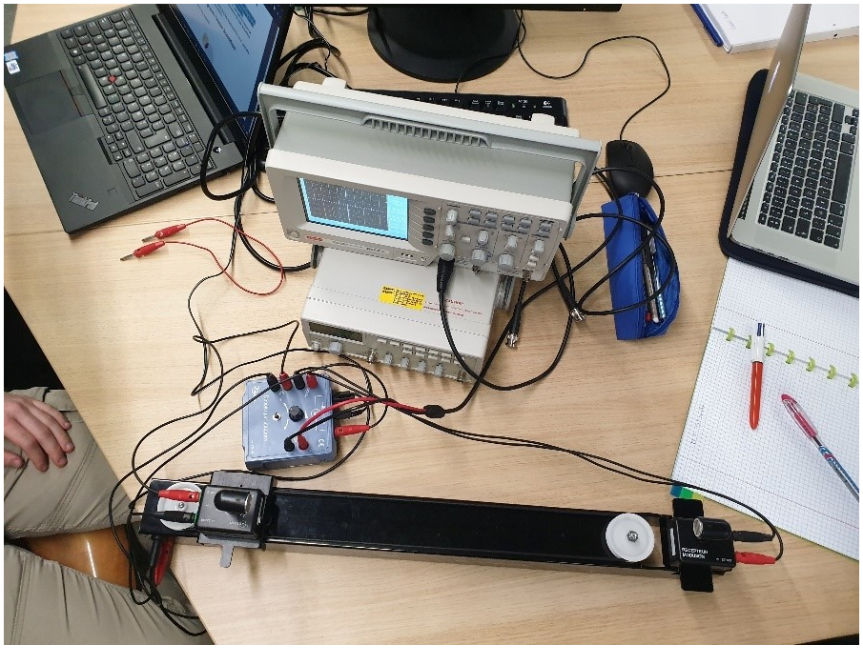
\includegraphics[width=0.85\textwidth]{montage-complet2.PNG}
    \caption{Montage complet.}
    \label{fig:montageComplet}
  \end{figure}
  \item Nous avons positionné l’émetteur en face du récepteur et nous avons relevé la fréquence du signal reçu. Nous pouvons faire la remarque sans mouvement de l’émetteur, la fréquence du signal émis est celle du signal reçu. À partir du signal en sortie du récepteur Moduson, nous avons relevé la période du signal émis.
\end{enumerate}
Pour une manipulation plus facile, nous avons positionné l’émetteur et le récepteur Moduson sur le banc de mécanique Doppler. Ils sont ainsi alignés sans effort.










\subsubsection{Calcul de la vitesse du chariot avec la relation de Doppler}





Notre émetteur utilise une fréquence de 40 kHz. Nous pouvons calculer la vitesse de déplacement de l’émetteur grâce à la relation de Doppler:
\[ v = c \times \frac{\Delta f}{f_{\text{ém}}} \]
où:
\begin{itemize}
  \item $c$ est la vitesse du son dans l’air (340 m/s),
  \item $\Delta f$ est la fréquence du signal ultrasonore en sortie du boîtier,
  \item $ f_{\text{ém}} $ est la fréquence du signal ultrasonore émis.
\end{itemize}
Après avoir appliqué cette formule, voilà ce que nous obtenons:
\begin{itemize}
  \item la vitesse la plus faible du chariot: 0,0578 m/s,
  \item la vitesse intermédiaire: 0,0935 m/s,
  \item la vitesse maximale à laquelle le chariot pouvait se déplacer: 0,140 m/s.
\end{itemize}
Calculons maintenant la vitesse mais en utilisant la formule classique de celle-ci, à savoir: $ v = m \times s $. Nous obtenons ces valeurs:
\begin{itemize}
  \item vitesse la plus faible: 0,059 m/s,
  \item vitesse intermédiaire: 0,107 m/s,
  \item vitesse maximale: 0,156 m/s.
\end{itemize}
Ici, la différence entre nos premières et nos secondes valeurs est due à 2 facteurs lié à l'imprécision dans la mesure lors de l’obtention de nos 2èmes valeurs. Tout d’abord, le temps compté pour chaque trajet, aussi vif que nous puissions l’être, ne sera jamais totalement vraie. Ensuite, la distance comptée n’est pas très précise non plus. Nous avons utilisé la valeur de 40 cm notée sur le flanc du banc mécanique. Or, cette distance correspond au côté le plus éloigné de l’émetteur par rapport au récepteur, jusqu’au côté de l’émetteur le plus proche du récepteur. Ce que nous pouvons constater sur la figure \ref{fig:quarantecm}.

\begin{center}
  \begin{figure}[H]
    \centering
    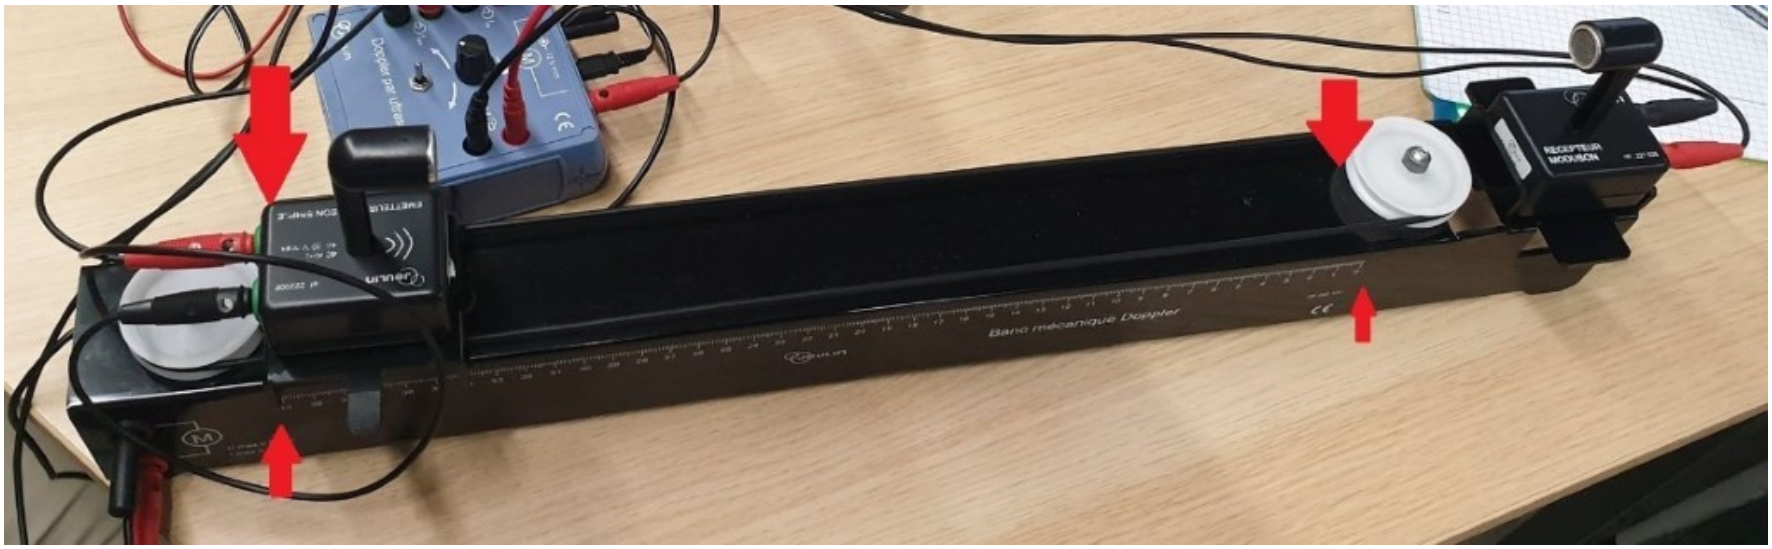
\includegraphics[width=0.95\textwidth]{40cm.PNG}
    \caption{Banc mécanique.}
    \label{fig:quarantecm}
  \end{figure}
\end{center}









\subsection{Câblage}










\subsubsection{Principe de la manipulation}





Dans le monde de l’informatique, il existe de multiples façons d’interconnecter des machines. La plus commune est bien évidemment le câble Ethernet. Dans la manipulation suivante, nous allons nous munir de plusieurs câbles ainsi que d’un testeur de câble qui va nous permettre entre autres de vérifier l’ordre des paires et donc de déterminer si le câble est droit ou croisé (voir section \ref{subsec:cables} pour un rappel théorique sur les câbles droits et croisés).










\subsubsection{Matériel utilisé}





\begin{itemize}
  \item Un testeur de câble.
  \item Des câbles avec différents PinOut.
\end{itemize}










\subsubsection{Problèmes rencontrés}





Au début de la manipulation, nous n’avions pas compris que le but était de visualiser l’ordre des paires. Ça nous a mené à connecter les câbles n’importe comment comme sur la figure \ref{fig:erreurCable1}, où sont connectés un câble vert \textbf{et} un noir.

\begin{center}
  \begin{figure}[H]
    \centering
    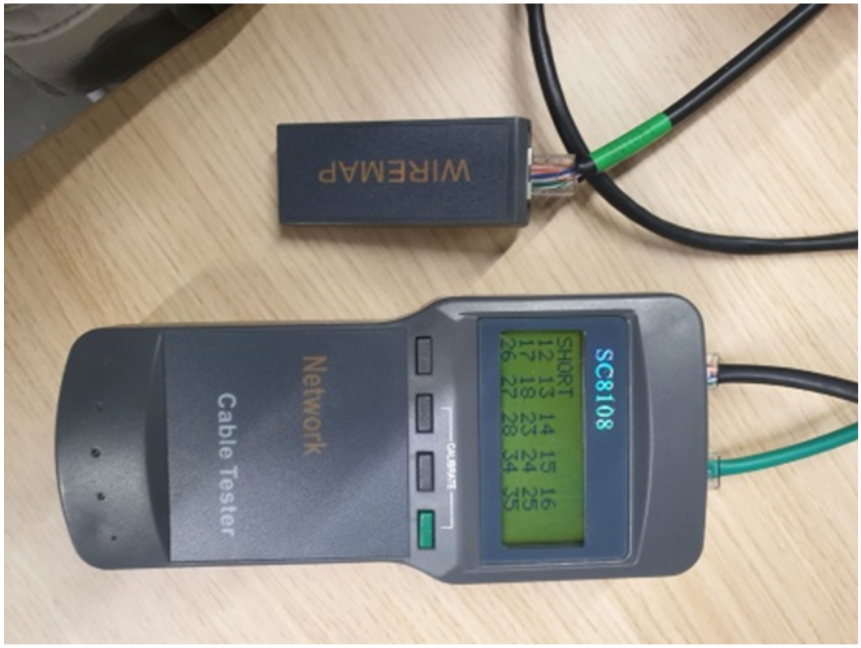
\includegraphics[width=0.75\textwidth]{erreur-cables1.PNG}
    \caption{Problème de compréhension dans le test des câbles.}
    \label{fig:erreurCable1}
  \end{figure}
\end{center}










\subsubsection{Résultats}





Après avoir compris comment fonctionnait le testeur de câble, nous avons testé deux câbles et voici ce qu’il en est ressorti:
\begin{itemize}
  \item Le premier câble que nous avons testé n’était ni droit, ni croisé et n’aurait jamais pu fonctionner. Comme on peut le voir sur la figure \ref{fig:failTestCable}, le test est FAIL.
  \begin{figure}[H]
    \centering
    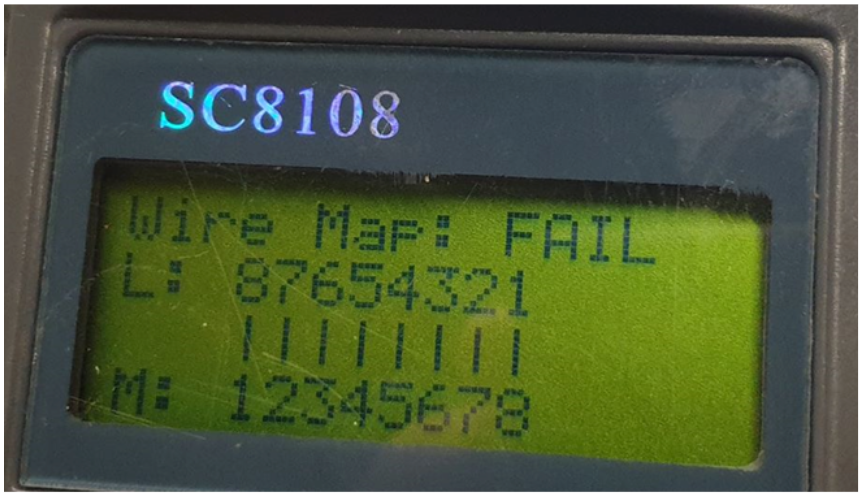
\includegraphics[width=0.75\textwidth]{fail-test-cable1.PNG}
    \caption{Test échoué.}
    \label{fig:failTestCable}
  \end{figure}
  \item Le deuxième câble, était quant à lui un câble droit, on peut voir dans la figure \ref{fig:passTestCable} que chaque pin est dans l'ordre et le test est PASS.
  \begin{figure}[H]
    \centering
    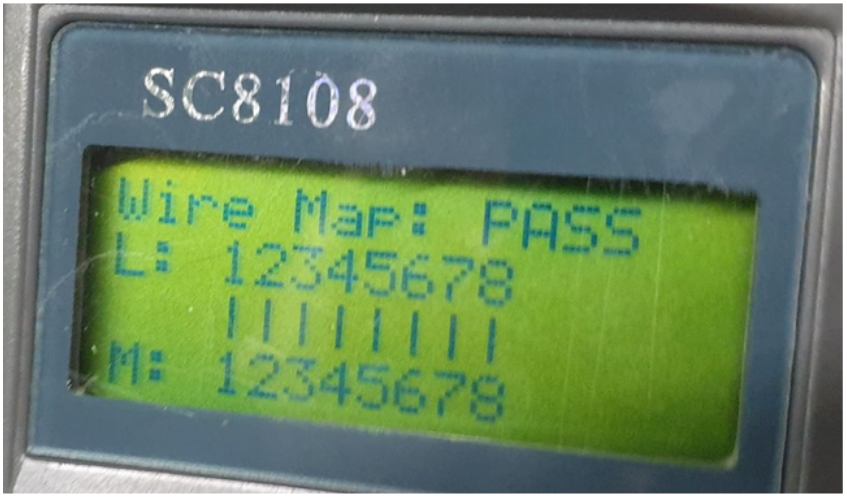
\includegraphics[width=0.75\textwidth]{pass-test-cable1.PNG}
    \caption{Test réussi.}
    \label{fig:passTestCable}
  \end{figure}
\end{itemize}
















\section{Conclusion}










\subsection{Conclusion sur l'effet Doppler}





Avec la manipulation du rail nous avons pu remarquer que les ondes peuvent prendre de multiples formes en fonction de certains paramètres. Ces paramètres sont les suivant: fréquence, vitesse, temps, distance.

La formule qui nous était donné dnas l'énoncé est la formule de Doppler:
\[ v = c \times \frac{\Delta f}{f_\text{ém}} \]
et nous avons pu vérifier par la pratique qu'elle était correcte en comparant les résultats donnés par cette formule (déterminée à partir de l’oscilloscope) et la vitesse calculée avec un chronomètre en connaissant la distance à parcourir (formule: vitesse = distance / temps).

La formule de Doppler permet de voir assez aisément que la vitesse influe sur la fréquence.










\subsection{Conclusion sur le câblage}





Grâce a cette manipulation nous avons découvert qu’il existe un appareil qui permet de tester la connectivité d’un câble. 

Il prend en compte plusieurs paramètres et les affiches:
\begin{itemize}
  \item Longueur de câble, un module distant si l’extrémité du câble se trouve trop loin pour brancher les 2 à l’appareil.
  \item La configuration des broches, affiche s’il y a bien une connexion correcte ou non entre l’émission et la réception.
  \item Déterminer si un câble est croisé ou droit.
  \item Les connexions ouvertes.
  \item Les courts-circuits.
\end{itemize}

\textbf{Remarque}: au premier coup d’œil on imagine difficilement toute les variables mesurées par cette appareil il a fallu se renseigner avant d’en comprendre l’utilité et le fonctionnement peu intuitif de l'appareil.














\end{document}
